\dev{Emile Martinez}{}{}{}

\subsection{Les piles}

\textbf{Rappel :} Une pile est une structure de données avec les méthodes \texttt{vide}, \texttt{est\_vide}, \texttt{empiler}, \texttt{depiler}.

\subsubsection{Implémentation par listes}

Cette manière est immédiate et donc naturelle.

\begin{exercise}[Au tableau avec participation des élèves]
	A quoi correspondent les opérations de bases de la pile sur une liste (à l'oral et éventuellement avec le dessin d'une liste simplement chaînés pour montrer les modifications).
\end{exercise}

Les listes étant naturelles en OCaml, nous les implémenterons de cette manière en Ocaml. Néanmoins cette pile est immuable.

\subsubsection{Implémentation par tableaux}

La deuxième manière est en utilisant un tableau. \\

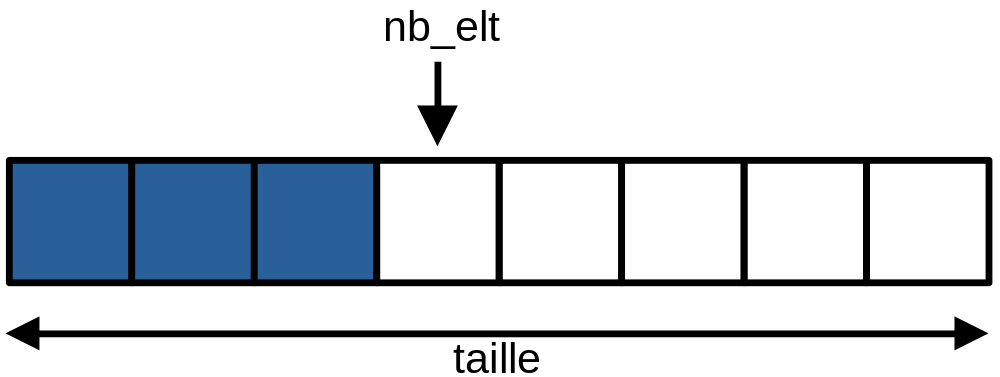
\includegraphics[scale=0.3]{lecon/05-piles_files/piles_tableau.png}
\\

\begin{principe}
	Pour cela, on utilise un indice \texttt{nb\_elt} qui nous indiquera à quelle case du tableau correspond le sommet de la pile, les cases précédentes du tableau contenant les autres éléments empilés.
\end{principe}

\begin{impl}
	On doit soit alors utiliser un tableau de taille fixe (et donc connaître à l'avance le nombre max d'éléments dans la pile)
\end{impl}